\section{Distribución geométrica y binomial negativa}
\subsection{La Distribución Geométrica}

La distribución geométrica modela el número de ensayos Bernoulli independientes necesarios para obtener el primer éxito. Si cada ensayo tiene probabilidad de éxito $p$ y de fracaso $q=1-p$, entonces la variable aleatoria $X$ que cuenta el número de ensayos hasta obtener el primer éxito (incluyendo el éxito) tiene función de probabilidad
\begin{align}
 \label{eq:2.10.9}
 f(k) = P(X=k) = (1-p)^{k-1}p, \quad k=1,2,3,\dots
\end{align}

Una propiedad fundamental de la distribución geométrica es la \emph{pérdida de memoria}: la probabilidad de obtener un éxito en los siguientes $k$ ensayos no depende del número de fracasos previos. Esto es, si $m,n\geq 1$,
\begin{align}
 P(X > m+n \mid X > m) = P(X > n).
\end{align}

{Propiedades de la distribución geométrica} Si $X$ tiene distribución geométrica con parámetro $p$, entonces
\begin{align}
 \mu_{X} &= \dfrac{1}{p} \\
 \s_{X}^{2} &= \dfrac{1-p}{p^{2}}.
\end{align}

\begin{ejemplo}
 \label{exmp:2.10.13}
 Un vendedor sabe que la probabilidad de cerrar una venta en cada llamada telefónica es $p=0.2$. ¿Cuál es la probabilidad de que necesite realizar exactamente $5$ llamadas para realizar la primera venta? ¿Cuántas llamadas se espera que necesite en promedio?
\end{ejemplo}

\begin{solucion}
	Usando la distribución geométrica con $p=0.2$:
	\begin{align}
		P(X=5) &= (1-0.2)^{5-1}(0.2) = (0.8)^{4}(0.2) \\
		&= 0.4096 \times 0.2 = 0.08192
	\end{align}

	El número esperado de llamadas es
	\begin{align}
		\mu = \dfrac{1}{p} = \dfrac{1}{0.2} = 5.
	\end{align}
\end{solucion}

\begin{ejemplo}
 \label{exmp:2.10.14}
 En un proceso de control de calidad, la probabilidad de que una pieza sea defectuosa es $p=0.1$. ¿Cuál es la probabilidad de que la primera pieza defectuosa aparezca en la tercera inspección?
\end{ejemplo}

\lstinputlisting[language=Python]{../code/distribuciones-especiales/distGeom.py}

\begin{figure}
 \centering
 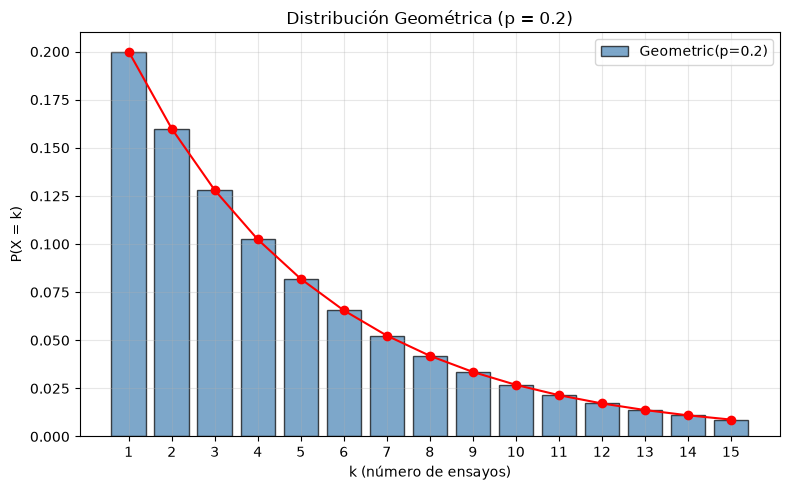
\includegraphics[height=7cm,keepaspectratio=true]{./pe/distGeom.png}
 % distGeom.png: 0x0 pixel, 300dpi, 0.00x0.00 cm, bb=
 \caption{Distribución geométrica con $p=0.2$}
 \label{fig:2.10.7}
\end{figure}



\subsection{La Distribución Binomial Negativa}

La distribución binomial negativa generaliza la geométrica: modela el número de fracasos observados antes de obtener un número predeterminado $r$ de éxitos en una secuencia de ensayos Bernoulli independientes. Su función de probabilidad está dada por
\begin{align}
 \label{eq:2.10.10}
 f(k) = P(X=k) = \binom{k+r-1}{r-1}p^{r}(1-p)^{k}, \quad k=0,1,2,\dots
\end{align}

Observe que cuando $r=1$, la binomial negativa se reduce a la distribución geométrica (contando fracasos antes del primer éxito).

{Propiedades de la distribución binomial negativa} Si $X$ tiene distribución binomial negativa con parámetros $r$ y $p$, entonces
\begin{align}
 \mu_{X} &= \dfrac{r(1-p)}{p} \\
 \s_{X}^{2} &= \dfrac{r(1-p)}{p^{2}}.
\end{align}

\begin{ejemplo}
 \label{exmp:2.10.15}
 Un examen de certificación tiene una tasa de aprobación del $30\%$. ¿Cuál es la probabilidad de que un estudiante repruebe $4$ veces antes de aprobar por tercera vez?
\end{ejemplo}

\begin{solucion}
	En este caso, $r=3$ (número de éxitos) y $p=0.3$. La variable $X$ cuenta el número de fracasos antes del tercer éxito.
	\begin{align}
		P(X=4) &= \binom{4+3-1}{3-1}(0.3)^{3}(0.7)^{4} \\
		&= \binom{6}{2}(0.027)(0.2401) \\
		&= 15 \times 0.027 \times 0.2401 \\
		&\approx 0.0972
	\end{align}
\end{solucion}

\lstinputlisting[language=Python]{../code/distribuciones-especiales/distNegBinom.py}

\begin{figure}
 \centering
 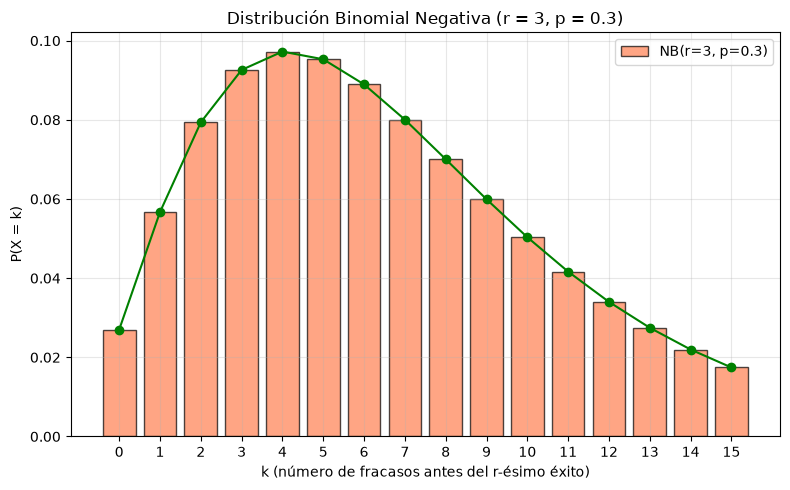
\includegraphics[height=7cm,keepaspectratio=true]{./pe/distNegBinom.png}
 % distNegBinom.png: 0x0 pixel, 300dpi, 0.00x0.00 cm, bb=
 \caption{Distribución binomial negativa con $r=3$, $p=0.3$}
 \label{fig:2.10.8}
\end{figure}


